% Created 2017-04-25 Tue 14:06
% Intended LaTeX compiler: xelatex
\documentclass[a4paper, notitlepage]{report}
\usepackage{graphicx}
\usepackage{grffile}
\usepackage{longtable}
\usepackage{wrapfig}
\usepackage{rotating}
\usepackage[normalem]{ulem}
\usepackage{amsmath}
\usepackage{textcomp}
\usepackage{amssymb}
\usepackage{capt-of}
\usepackage{hyperref}
% set the margins here, if they need to be modified
\usepackage[a4paper, left=1.3in, right=1.0in]{geometry}

\usepackage[style=ieee,backend=biber]{biblatex}

% The linespacing you want
\linespread{1.4}

% Lets you pick fonts. Only works if you compile with xelatex or luatex
\usepackage[no-math]{fontspec}

\usepackage{unicode-math}

\usepackage{stackengine}
\stackMath

% Used to make the captions on figures sans serif
\usepackage{caption}

% For including images
\usepackage{graphicx}
\usepackage{float}

\usepackage{color}

% For fancy code listings
\usepackage{minted}
\usemintedstyle{emacs}

% For tables that span multiple pages elegantly
\usepackage{longtable}

% For maintaining a list of abbreviations
\usepackage{nomencl}

% For drawing diagrams
\usepackage{tikz}

% These closely match the SCSS word template fonts
% Won't work unless you compile with xelatex or luatex
\setmainfont[Mapping=tex-text]{Times New Roman}
\setsansfont{Helvetica}
\setmonofont[Scale=MatchLowercase]{Monaco}
\setmathfont{TeX Gyre Termes Math}

\hypersetup{
  colorlinks,
  citecolor=black,
  filecolor=black,
  linkcolor=black,
  urlcolor=black
}

% Change these as appropriate, and they'll be filled in automatically on the
% cover page. You can also use them throughout the document, so as not to have
% to type them again all the time.
\newcommand \authorname{Eoin Houlihan}
\newcommand \authoremail{ehoulih@tcd.ie}
\newcommand \supervisorname{Dr. Glenn Strong}
\newcommand \degreetitle{B.A.(Mod.) Computer Science}
\newcommand \projecttitle{Dependent Types in Practice}

% All the commands are defined in this file
\newcommand \inserttitlepage{\thispagestyle{empty}
\begin{center}
{\sffamily
{\Large University of Dublin}

\vspace{10pt}


\includegraphics[scale=0.12]{tcd/trinitycollege.pdf}

\vspace{10pt}

{\Huge TRINITY COLLEGE}

\vspace{80pt}

\textbf{ \Large \emph \projecttitle}

\vspace{30pt}

\authorname

\degreetitle

Final Year Project May 2017

Supervisor: \supervisorname

\vspace{130pt}

\large{School of Computer Science and Statistics
\\$ $\\
O'Reilly Institute, Trinity College, Dublin 2, Ireland}
\linespread{1}
}
\end{center}
}
\newcommand \insertabstract{\begin{abstract}
\thispagestyle{plain}
Major software vulnerabilities in critical software have led to more interest in
formal verification of our software. One way that has presented itself to verify
our code is by using dependent types, an idea from the 1970s present in a number
of upcoming programming languages and interactive theorem provers.

We present a study into the current state-of-the-art dependently-typed
programming languages. Idris was chosen as the tool to carry out this study. The
methodology involved carrying out case studies of applying dependent types to
real-world programming problems. An evaluation of the outcomes and the current
landscape of dependently-typed programming languages applied in a practical
sense is provided as a result of carrying out these case studies.
\end{abstract}
}
\newcommand \declaration{\chapter*{Declaration}

I hereby declare that this project is entirely my own work and that it has not
been submitted as an exercise for a degree at this or any other university.
$ $\\
$ $\\
\signed{\authorname}
}
\newcommand \acknowledgements{\chapter*{Acknowledgements}
Firstly, I would like to thank my parents for giving me the opportunity, support
and encouragement I needed throughout my degree.

\noindent
I would like to thank Glenn Strong for his continued guidance and suggestions
throughout this project as my supervisor.

\noindent
I would also like to thank the budding Idris and dependent type community,
particularly those in the \#idris IRC channel, for being patient enough to
answer any questions that I had.
}
\newcommand \permissiontolend{\chapter*{Permission to lend}

I agree that the Library and other agents of the College may lend or copy
this report upon request.

$ $\\
$ $\\
\signed{\authorname}
}
\newcommand \ibidp{(\emph{Ibid.})}
\newcommand \ibid{\emph{Ibid.}}

\newcommand{\argmax}[1]{\underset{#1}{\operatorname{arg}\,\operatorname{max}}\;}

\usepackage{datetime}

\def\fullhrulefill{\leavevmode\leaders\hrule height 1pt\hfill\kern 0pt}

\newcommand{\signedanddate} {
  \par\noindent\makebox[2.5in]{\fullhrulefill}
  \par\noindent\makebox[2.5in][l]{\authorname, May 5 2017}
}

\newcommand \needcite[1]{\underline{#1}}

\newcommand \abbrev[2]{#1\nomenclature{#1}{#2}}


% For changing the names of the List of Listings, etc.
\renewcommand*{\contentsname}{Table of Contents}
\renewcommand*{\nomname}{Abbreviations}

% Make the captions sans serif
\renewcommand{\captionfont}{\sffamily}

\addbibresource{report.bib}
\author{Eoin Houlihan}
\date{\today}
\title{Dependent Types in Practice}
\hypersetup{
 pdfauthor={Eoin Houlihan},
 pdftitle={Dependent Types in Practice},
 pdfkeywords={},
 pdfsubject={},
 pdfcreator={Emacs 25.2.1 (Org mode 9.0.5)},
 pdflang={English}}
\begin{document}

\inserttitlepage
\pagenumbering{roman}
\declaration
\permissiontolend
\insertabstract
\acknowledgements
\tableofcontents
\newpage
\pagestyle{headings}
\pagenumbering{arabic}

\chapter{Introduction}
\label{sec:org3d8a24c}
\chapter{Background}
\label{sec:orgd9fb8aa}
This chapter aims to give an understanding of the background and necessary
concepts that will be used throughout the report. A basic understanding of
functional programming ideas such as algebraic data types, recursion and the
fundamentals of the Hindley-Milner type system with respect to languages such as
Haskell is assumed of the reader. It also gives a broad overview of the current
state of the art dependently-typed programming languages with a more in-depth
look at Idris in particular.

\section{Intuitionistic Type Theory}
\label{sec:orge35e0cc}
Intuitionistic type theory is a type theory based on mathematical
constructivism. Constructive mathematics is an alternative foundational theory
of mathematics that argues that construction of a mathematical object is
necessary to proving that such an object exists. Of particular note, the
intuitionistic logic which much of constructivism uses deviates from classical
logic systems in that proof by contradiction is not used and the law of the
excluded middle is not assumed as an axiom of the logic in general.

Drawing upon these ideas, Per Martin-Löf, a Swedish logician, developed a number
of successive type theories in the 1970s \cite{martin-lof_intuitionistic_1984}.
This intuitionistic type theory (also commonly referred to as Martin-Löf type
theory) introduces a number of interesting concepts. Most notable in terms of
their influences on programming language design were the concepts of \(\Pi\)-types
and \(\Sigma\)-types. These constructs can be seen as analogous to the logical
quantifiers ``forall'' and ``exists'' respectively. These concepts have served
as the underpinning of the development of dependently-typed programming
languages and theorem provers based on Martin-Löf type theory.

\section{Curry-Howard Isomorphism}
\label{sec:orgb6da51e}
From a modern computer science perspective it's almost taken for granted that
computability theory and mathematical proofs are inherently linked. For example,
many parallels can be drawn between the proof of Turing's Halting Problem and
Gödel's incompleteness theorems. Between the 1930s and the 1960s Haskell Curry
and William Alvin Howard began to formalise this direct link between computer
programs and mathematical proofs which is known as the Curry-Howard isomorphism
\cite{mcadams_tutor_2013}. As Philip Wadler, one of the original authors of the
Haskell report, put it \cite{strange_loop_2015,wadler_propos_2015}

\begin{quote}
``Every good idea will be discovered twice. Once by a logician and once by a
computer scientist'' -- Philip Wadler
\end{quote}

According to the Curry-Howard isomorphism the type of an expression is
equivalent to a proposition of a logical formula. A term inhabiting that type is
therefore equivalent to a proof that the proposition holds. Some concrete value
exists that bears witness to the type being inhabited. In other words, a proof
can be constructed. This very much aligns with the constructivist view of
mathematics. Other correspondences can be shown such as between logical
implication and function types, conjunction and product types and between false
formulas and the uninhabited type, bottom (\(\bot\)). We can even see from the
shape of the syntax rules of both natural deduction and simply-typed lambda
calculus that these kinds of correspondences exist. As an example, the
relationship between the Modus Ponens rule and the function application rule.
\[ \scalebox{2}{$\frac{\Gamma \vdash \alpha \rightarrow \beta \qquad \Gamma
\vdash \alpha}{\Gamma \vdash \beta} \rightarrow E \qquad \frac{\Gamma \vdash
t:\alpha \rightarrow \beta \qquad \Gamma \vdash u:\alpha}{\Gamma \vdash
t\;u:\beta}$} \]

One of the consequences of this relationship is the possibility of a unification
at a primitive level between mathematical logic and the foundations of
computation. In practical terms this relationship has influenced the work on
programming languages such as Coq and Idris that allow proofs to be written as
programs that can be formalised, verified and executed. This is interesting to
the practice of software engineering as it gives us the power to reason about
program correctness by translating a mathematical proof of an algorithm to a
computer program and having the machine type-check (proof-check) it.

\section{Traditional Hindley-Milner Type Systems}
\label{sec:orgcbb824c}
Standard Hindley-Milner-esque type systems such as the one found in Haskell
allow us to express some different dependencies between the types of terms and
terms themselves. For example, terms can depend on other terms such as in this
Haskell function definition.

\begin{listing}[H]
\begin{minted}[frame=single,fontsize=\normalsize,linenos,breaklines,escapeinside=\#\#]{haskell}
plusOne x = x + 1
\end{minted}
\caption{A simple Haskell function definition (terms depending on terms)}
\end{listing}

Here we can see that the term \texttt{plusOne} has been defined with respect to the
terms \texttt{x}, which is its argument and \texttt{1}, an integer. Types can also depend on
other types as shown here.

\begin{listing}[H]
\begin{minted}[frame=single,fontsize=\normalsize,linenos,breaklines,escapeinside=\#\#]{haskell}
data List a = Nil
            | Cons a (List a)
\end{minted}
\caption{A Haskell data type definition with a type parameter (types depending on types)}
\end{listing}

In this Haskell data type definition, the type constructor \texttt{List} depends on the
type \texttt{a} provided to it. This allows polymorphism and lists of any type.
Finally, in the world of Haskell, terms can depend on types. This is apparent in
polymorphic functions such as the identity function.

\begin{listing}[H]
\begin{minted}[frame=single,fontsize=\normalsize,linenos,breaklines,escapeinside=\#\#]{haskell}
id :: a -> a
id x = x
\end{minted}
\caption{A polymorphic Haskell function definition (terms depending on types)}
\end{listing}

\section{Dependent Type Systems}
\label{sec:org9084189}
Dependent type systems extend this system of dependencies by allowing types to
depend on terms. This leads to much greater expressivity power in the type
system. For example, in a dependently typed system we can express types such as
the type of pairs of natural numbers where the second number is greater than the
first.

If we take the view of the Curry-Howard isomorphism that types are propositions
and terms are witnesses to a proof of that proposition then we can see the
advantages of a more expressive type system. We can now encode much more
sophisticated propositions in the type system and if we can prove them (i.e.
construct a value that inhabits that type) then we can guarantee much more
interesting correctness properties about the code that we are writing. For this
reason, dependent types have seen much use in the areas of formal verification
of computer programs and formal computer encoding of mathematical objects and
proofs.

There are 3 main concepts taken from Martin-Löf type theory and implemented in
dependently-typed programming languages.

\subsection{\texorpdfstring{$\Pi$}{Pi}-types}
\label{sec:orgafe9307}
\(\Pi\)-types are the types of functions whose return types depend on one or more of
their arguments. In other words these functions map values from some domain to
some non-fixed codomain that is determined by the input. In this sense the
return type is said to be dependent upon the input.

If we have a representation of \(n\textrm{-tuples}\) of some type \(A\),
\(\operatorname{Vect}(A,n)\), then the \(\Pi\)-type \(\Pi_{(n \mathbin{:} {\mathbb N})}
\operatorname{Vect}(A,n)\) represents the type of functions that given some
natural number \(n\) return a tuple of size \(n\) of elements of type \(A\). That is
to say that the type of the value returned by these functions is determined by
the argument to the functions.

\subsection{\texorpdfstring{$\Sigma$}{Sigma}-types}
\label{sec:org7ca43af}
\(\Sigma\)-types, also known as dependent pair types, are a more generalised form of
Cartesian product that model pairs of values where the type of the second
element depends on the first element.

Again using the \(\operatorname{Vect}\) representation of \(n\textrm{-tuples}\) of
some type \(A\), the \(\Sigma\)-type \(\Sigma_{(n \mathbin{:} {\mathbb N})}
\operatorname{Vect}(A,n)\) represents a pair of a natural number \(n\) and a tuple
of length \(n\) of values of type \(A\).

This representation is similar to the Haskell \texttt{List} type however there is extra
information in that the type of the \(\Sigma\)-type \(\operatorname{Vect}\) also
carries around a witness to its length expressed as a natural number. We say
that \(\operatorname{Vect}\) is ``indexed'' by the type \(A\) as well as the value
\(n\).

Being able to index types by both types and terms in the language is a key
feature of dependently-typed programming languages. These languages eliminate
the distinction between types and terms. Types and terms are unified as
equivalent constructs.

\subsection{The Equality Type}
\label{sec:org345c71c}
The equality type \(=\) is a special type used to denote proofs of equality
between two values. If there is an inhabitant of the type \(a \mathrel{=} b\) then
\(a\) and \(b\) are considered to be equal. This proof allows \(b\) to be used
anywhere \(a\) would have been used. There is only one inhabitant of the type \(a
\mathrel{=} a\), the reflexive proof of equality.

\[ \scalebox{2}{$\operatorname{refl} \mathbin{:} \Pi_{(a \mathbin{:} A)} (a
\mathrel{=} a)$} \]

This type is particularly useful in dependently-typed programming in that it can
be used as a witness that two terms are equivalent and allows a substitution of
one term for another to take place. With it, we can begin to develop
constructions of basic proofs and axioms such as \(n \mathbin{:} {\mathbb N}, n
\mathbin{-} n \mathrel{=} 0\).

\section{State of The Art Dependently-Typed Programming Languages}
\label{sec:org721c0c0}
\subsection{Agda}
\label{sec:org53bcde7}
Originally developed in the late 1990s by Catarina Coquand and subsequently
rewritten by Ulf Norell in 2007, Agda is a dependently typed programming
language with support for features such as dependent pattern matching and
definition of inductive data types.

For example, the inductive data type representing the Peano natural numbers can
be declared as follows in Agda.

\begin{listing}[H]
\begin{minted}[frame=single,fontsize=\normalsize,linenos,breaklines,escapeinside=\#\#]{agda}
data #$ℕ$# : Set where
  zero : #$ℕ$#
  suc : #$ℕ$# → #$ℕ$#
\end{minted}
\caption{Agda definition of a natural number type}
\end{listing}

There are two cases to consider here. \texttt{zero} is the base case. \texttt{suc} (standing
for successor) takes a natural number and returns a new natural number. It
represents a natural number plus 1. We will see more definitions of inductive
types similar to this one throughout the later chapters.

Agda has the capability of producing executable code however it is mostly used
for the purpose of automated theorem proving. Agda does however provide a
foreign function interface to import arbitrary Haskell types and functions.
These go unused for the purpose of Agda type-checking but do have runtime
effects in the output compiled code.

\subsection{Coq}
\label{sec:org4d7175a}
Developed initially in the late 1980s at INRIA in France, Coq approaches
dependently-typed programming more from the mathematical side as an interactive
theorem prover. Coq is based on the Calculus of Constructions, a type theory
created by Thierry Coquand. Coq provides useful facilities for defining
inductive data types and includes a tactics language for doing interactive
proofs.

Notable work created using Coq includes the formally verified C compiler
CompCert \cite{leroy_compiler_2009}, as well as a formally verified proof of the
Four-Colour Theorem \cite{gonthier_formal_2008} for graph colouring.

Development in Coq and using dependent types in general can become quite
complex. To support the powerful type system a number of featureful interactive
environments such as CoqIDE and Proof General \cite{proof_general} exist. These
environments provide semantic information about your code. This includes the
current environment of defined values as well as their types and the type of the
current goal that you are attempting to prove.

\begin{figure}[H]
\centering
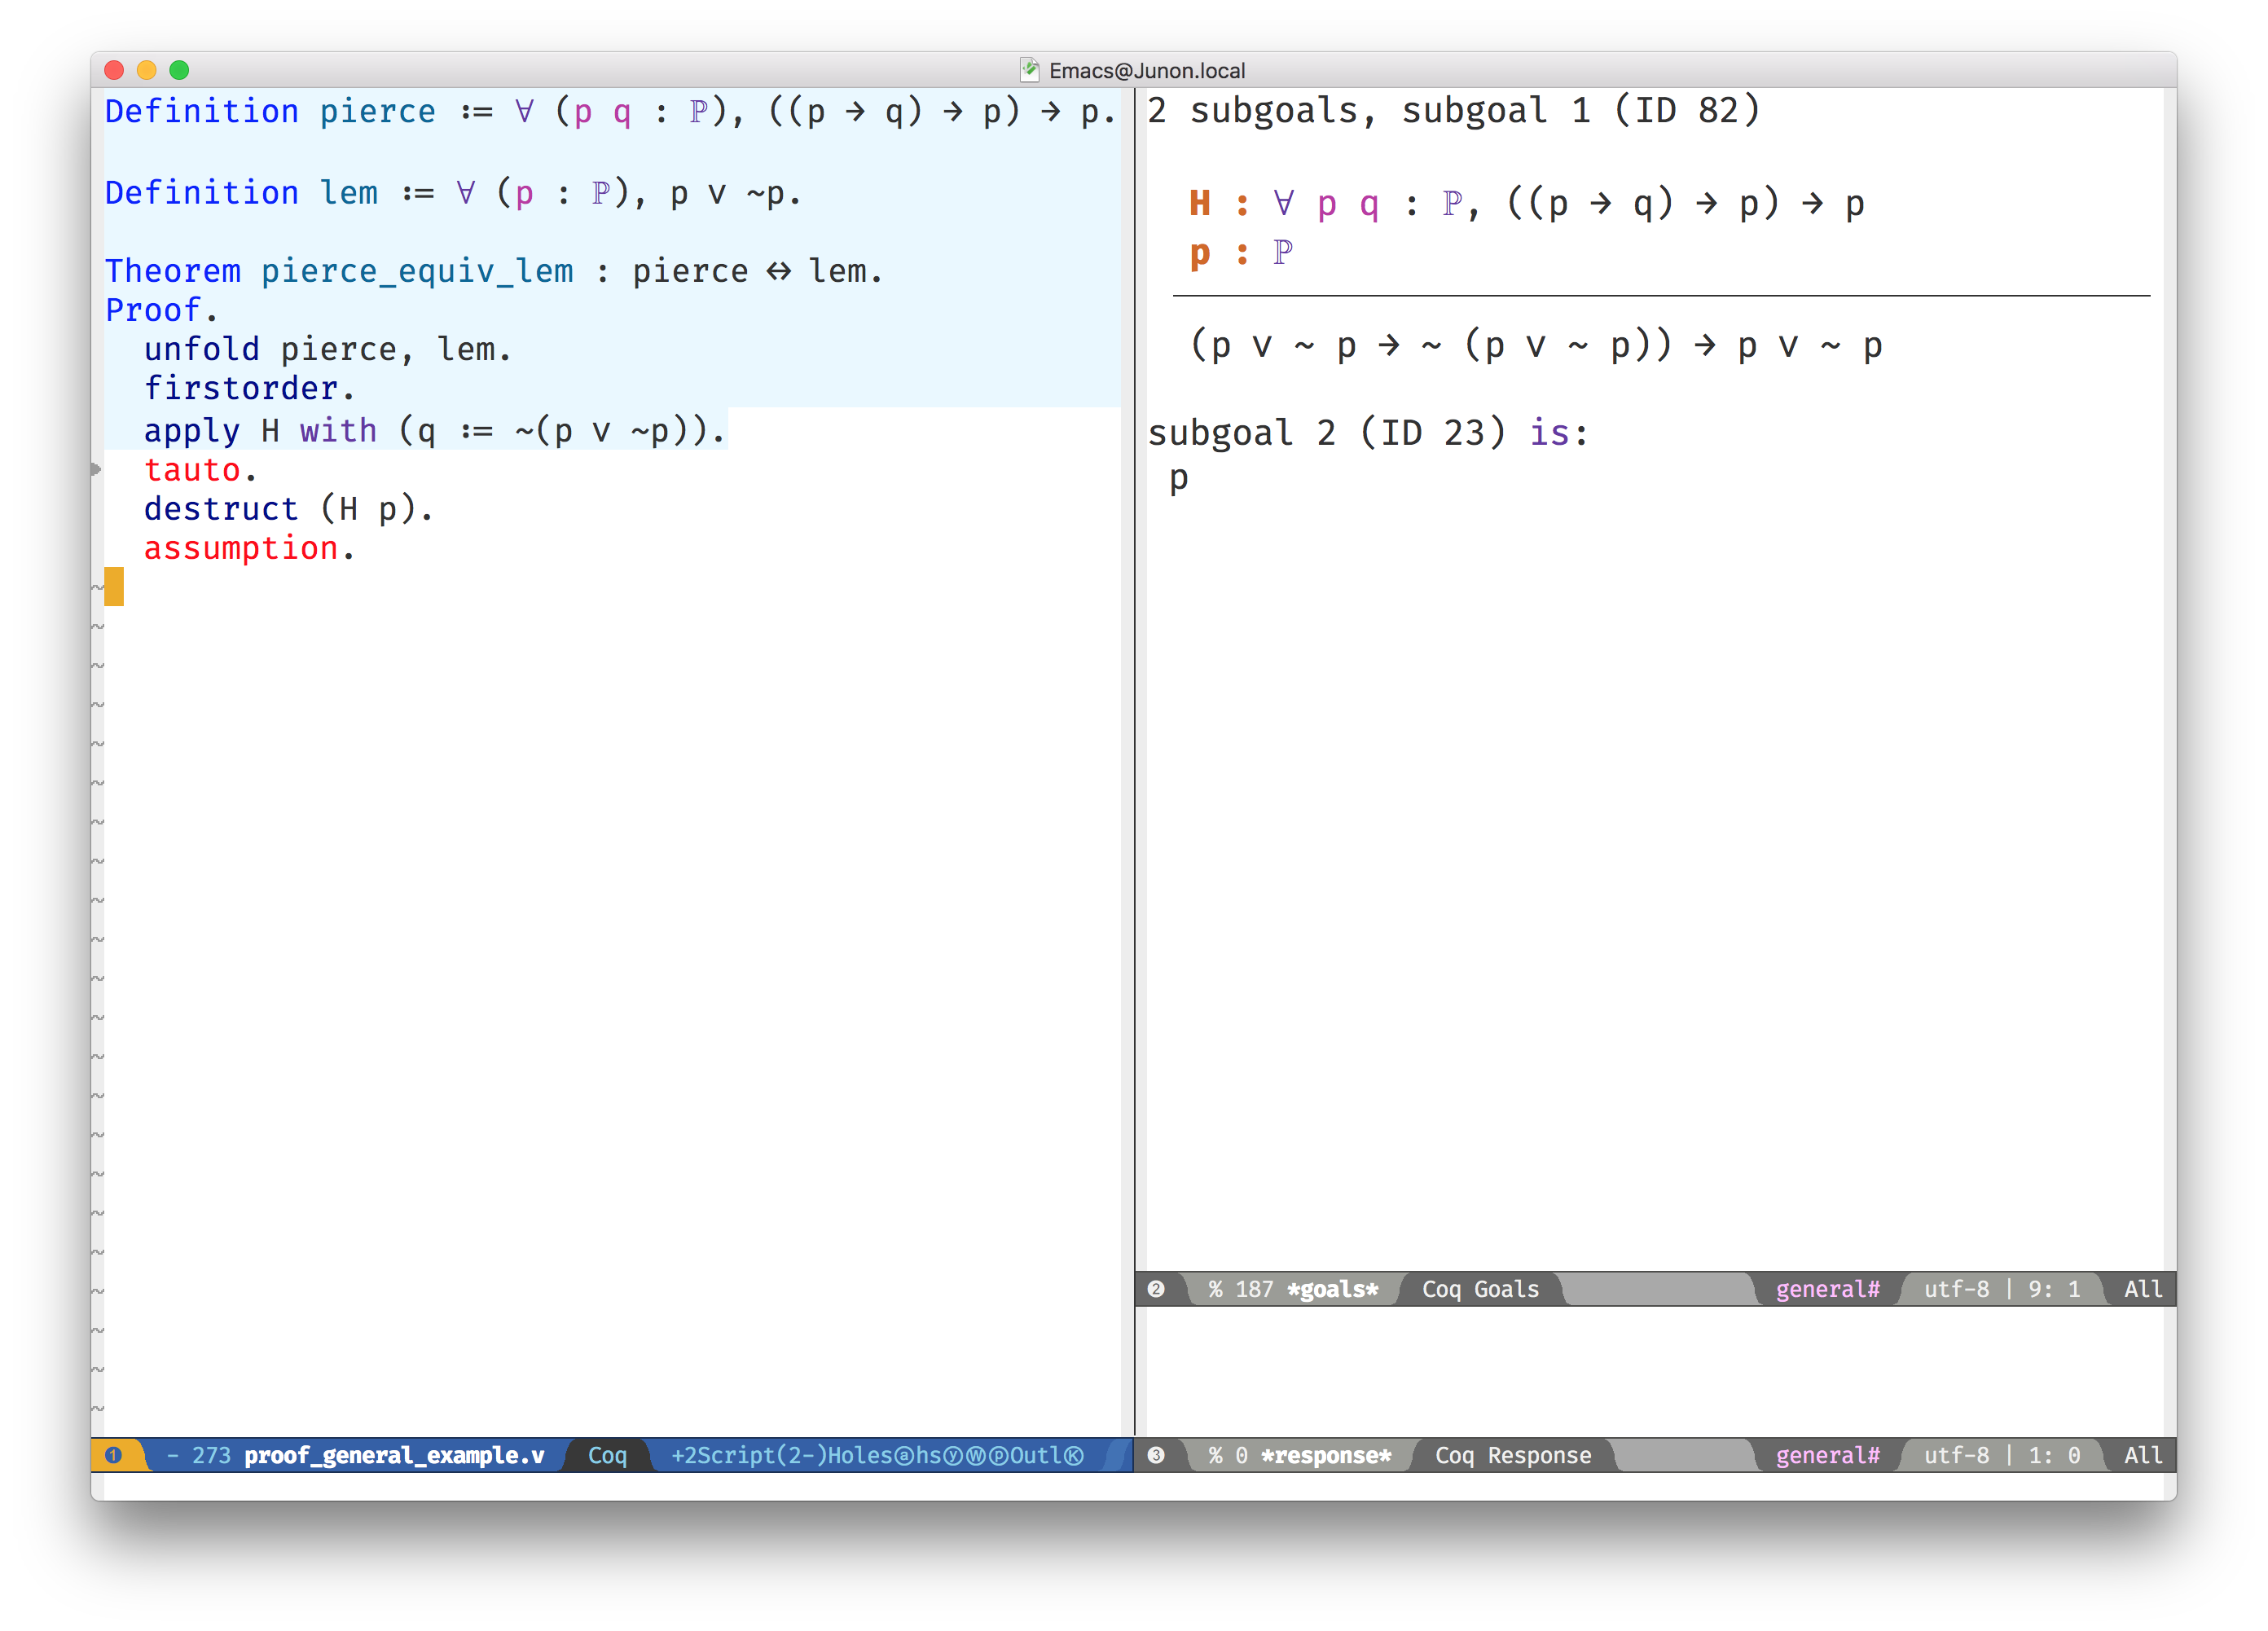
\includegraphics[width=0.85\linewidth]{./fig/proof_general.png}
\caption{An in-progress Proof General session}
\end{figure}

Coq's primary mechanism for producing executable code is via program extraction.
This is the process by which correct Coq code can be transformed into an
equivalent Haskell or OCaml module which provides the user with the ability to
run the extracted code. This extraction process has benefits in that it allows
for the expression and type-checking of interesting correctness properties in a
dependently-typed language while also giving us a way to compile it to native
code using compilers with state-of-the-art code optimisation techniques. This
allows the production of a fast native binary from a correct and type-checked
Coq program.

\subsection{Haskell}
\label{sec:org9a8b6a4}
GHC Haskell has slowly been implementing many of the capabilities of dependent
types via extensions to the language such as \texttt{GADTs}, \texttt{DataKinds}, and
\texttt{TypeFamilies}. Through particular use of the Haskell type system many of the
features of dependently-typed languages can be simulated in roundabout ways
\cite{mcbride_faking_2002,lindley_hasochism_2013}.

A full dependent type system is currently being implemented for future releases
of GHC 8 \cite{eisenberg_dependent_2016,weirich_specif_2017}. Existing
extensions and offshoots of GHC such as Liquid Haskell implement refinement
types which allows for the expression of a limited set of propositions at the
type level in existing Haskell code \cite{vazou_refinement_2014}.

\subsection{Idris}
\label{sec:org26c9f07}
Idris is primarily the work of Edwin Brady and others at the University of St
Andrews in Scotland. It has positioned itself as a more practical take on
dependently-typed programming and as such is more aimed at being a language that
you can write programs leveraging dependent types while also performing
interesting effectful actions such as file I/O and drawing graphics to the
screen.

Edwin Brady, the author of Idris has jokingly put it before that Idris has the
interesting property of being ``Pac-Man Complete'' \cite{scala_world_2015}. Idris
is not just a Turing complete language as everything from the x86 MOV
instruction to C++ templates turn out to be. Rather, if you wanted to, you could
write a version of a simple 2D game such as Pac-Man in the language with bitmap
graphics, animations, and sounds.

Idris provides multiple code generation backends to its compiler to produce
executable code. The primary mechanism by which code is generated is by using
the default C backend. This backend produces C code which is in turn compiled to
native code by a C compiler toolchain such as GCC or Microsoft Visual C++. Other
more experimental backends are provided such as JavaScript/Node.js as well as
community provided backends of the compiler such as the Erlang
\cite{elliott_erlang_2015} and Java \cite{idris_java} backends.

This report focuses on using Idris in a practical manner while aiming to take
advantage of dependent types to ensure that our code is more correct.
\chapter{Project Objectives and Approach}
\label{sec:orgc954dfd}

\section{Objectives}
\label{sec:org3a80f88}
The objectives of this project are the following:
\begin{itemize}
\item Evaluate the practicality of dependently-typed programming languages
\item Evaluate Idris in particular in this regard
\item Understand what kinds of correctness properties can be expressed
\item Understand the scale at which formal verification with dependent types can be
applied in a software project
\item Explore and evaluate multiple approaches to building software with dependent
types
\item Discover the main pain points of approaching this style of development as
someone with functional programming experience in some ML family language
\end{itemize}

\subsection{Practicality of Dependently-Typed Programming Languages}
\label{sec:org22cd608}
Much of the literature about dependent types has been focused on advancing
research in the study of the theory of the field. This has manifested itself by
way of new or novel approaches to building dependently-typed systems. Despite
the push to advance the underlying theory and concepts not much research has
emerged in the area of evaluating these languages' applicability to software
engineering as practised by programmers in general.

Some research exists such as Wouter Swierstra's 2012 evaluation
\cite{swierstra_xmonad_2012} of program extraction from Coq to Haskell of a
drop-in replacement for one of the modules of the xmonad window manager. This
projects aim to further supplement this area of study with more data taking into
account the state-of-the-art at the time of writing.

\subsection{Expression of Correctness Properties}
\label{sec:orge87d51d}
Many of the current teaching examples involving dependent types present fairly
simple examples of correctness properties. In order to provide a cohesive
example that illustrates one or two points this is understandable.

This project aims to outline some more in-depth example of expressing
complicated correctness properties. By doing this we to understand what some of
the limitations are in terms of the expressivity of specification of a dependent
type as well as the feasibility of implementing a program to that specification.

\subsection{Scale of Applicability of Dependent Types}
\label{sec:orgdbf5c20}
In real-world settings in a software engineering project we are often faced with
certain time, performance and other delivery constraints. Projects do not have
unlimited time to work with crafting and deploying a perfectly verified piece of
software. While dependent types can give us more guarantees about the
correctness of our programs that doesn't mean that we will be able to deliver a
fully verified system within real-world constraints such as deadlines.

This project aims to understand where dependent types are most suited to being
applied both in terms of problem domains as well as scale. The aim is to see if
the biggest return on investment will be in verifying critical algorithms and
processes within a system, verifying a system at the boundaries between
subsystems or by applying formal verification using dependent types across an
entire system.

\subsection{Development Approaches when using Dependent Types}
\label{sec:orgd4bbac2}
A number of development approaches exist when using dependent types. One could
take a bottom-up approach in that existing code that has no existing correctness
properties is given some and then the proof obligations are discharged from the
implementation out to the type signature. Another approach that is seeing more
traction is the top-down type-driven or proof-driven development style. This
approach starts by deciding on a specification in a type and driving the
implementation based on that specification. This approach is outlined fully in
its own section of the report.

Among the project's aims is to see how these approaches can be applied to the
case studies and to determine where one might favour one approach over the other
for a particular problem.

\subsection{Pain Points when using Dependent Types}
\label{sec:org839efbc}
Current dependently-typed languages such as Agda and Idris bear much surface
syntax similarity to ML family languages such as Haskell. However, past these
surface details the underlying type frameworks differ quite a bit. Even with
experience and a good knowledge of a language like Haskell there will be many
pain points when learning how to use dependent types. This project aims to
detail some of these hurdles that will be common when beginning to use these
type systems.

\section{Approach}
\label{sec:orge5178f6}
The approach by which the evaluation of the above objectives took place is by
implementing a number of case studies. In order for these case studies to have
significant meaning they were focused on implementing real world algorithms that
have interesting correctness properties that can be expressed about them.

In the implementation of these case studies multiple software engineering tools
and approaches were used. This included trying to implement the case studies
using different levels of correctness guarantees. It also meant that the case
studies should be implemented with different engineering approaches such as the
top-down type-driven approach and the bottom-up approach where correctness
properties are validated after the program has been implemented. The case
studies also made use of different tooling such as working with standard tools
like text editors as well as more semantically rich interactive editing
environments.
\chapter{Idris and Type-Driven Development}
\label{sec:orgd58849e}
In order to follow along with some of the code examples it is worth gaining an
understanding of some of the basic principles of the Idris language. This
section is by no means comprehensive both in terms of the contents of this
report as well as the language as a whole but will make it easier to understand
the code fragments in later sections. More advanced concepts will be covered as
we encounter them throughout the report. A more thorough reference and tutorial
can be found on the Idris website \cite{idris_tutorial_2017} as well as in Edwin
Brady's ``Type-Driven Development with Idris'' \cite{brady_book_2017} book.

\section{Similarities to Haskell}
\label{sec:org9089225}
Idris has inherited much of the surface syntax of Haskell and will be quite
familiar to anyone who has worked in Haskell or a similar ML-like language
before. For example, the function that calculates the length of the list would
look as follows in Haskell.

\begin{listing}[H]
\begin{minted}[frame=single,fontsize=\normalsize,linenos,breaklines,escapeinside=\#\#]{haskell}
length :: [a] -> Integer
length [] = 0
length (_:xs) = 1 + length xs
\end{minted}
\caption{Basic Haskell function definition syntax \label{length-haskell}}
\end{listing}

An equivalent Idris function bears some resemblance with notable exceptions
being the explicit name \texttt{List} as the list type constructor and the swapping of
the type operator (\texttt{::}) and the cons operator (\texttt{:}).

\begin{listing}[H]
\begin{minted}[frame=single,fontsize=\normalsize,linenos,breaklines,escapeinside=\#\#]{idris}
length : List a -> Integer
length [] = 0
length (_::xs) = 1 + length xs
\end{minted}
\caption{Translation of Listing \ref{length-haskell} into Idris}
\end{listing}

Data-type declarations also follow a similar syntax with Idris code favouring
the explicit type signature style seen in Haskell GADTs. As an example we could
have a simple data type such as a list implemented in Haskell.

\begin{listing}[H]
\begin{minted}[frame=single,fontsize=\normalsize,linenos,breaklines,escapeinside=\#\#]{haskell}
data List a = Nil
            | Cons a (List a)
\end{minted}
\caption{Definition of a simple Haskell data type \label{list-haskell}}
\end{listing}

In Idris we could define it the same way however the idiom is to use the
explicit type signatures as it becomes the only way to implement more powerful
dependently-typed data types later on.

\begin{listing}[H]
\begin{minted}[frame=single,fontsize=\normalsize,linenos,breaklines,escapeinside=\#\#]{idris}
data List : Type -> Type where
  Nil : List a
  Cons : a -> List a -> List a
\end{minted}
\caption{Translation of Listing \ref{list-haskell} into idiomatic Idris}
\end{listing}

\section{Typed Holes}
\label{sec:orgfb979fd}
Often when writing code with heavily polymorphic and dependent types it can
become difficult to see how exactly the types should line up. Idris has a
built-in syntax for declaring typed holes which are a useful tool to help
dealing with the way these types line up.

Typed holes act as placeholders for a value of any type. At any point in the
program a typed hole can be introduced instead of a value. When we go to type
check our code the compiler will tell us the type of the value that the hole
needs to be replaced by. This allows the user to incrementally fill in values of
the correct type or defer writing the value that fits the type until later.

All Idris typed holes are identifiers that begin with a ``?'' such as
\texttt{?length\_rhs\_1}. In the following example, the compiler informs us when we load
the module that the type of both \texttt{?length\_rhs\_1} and \texttt{?length\_rhs\_2} is \texttt{Integer}.

\begin{listing}[H]
\begin{minted}[frame=single,fontsize=\normalsize,linenos,breaklines,escapeinside=\#\#]{idris}
length : List a -> Integer
length [] = ?length_rhs_1
length (x :: xs) = 1 + ?length_rhs_2
\end{minted}
\caption{Typed holes can stand in as expressions of any type in our definitions}
\end{listing}

As seen here, typed holes can appear anywhere in an expression such as the
right-hand-side of the \texttt{+} operator. Using typed holes to defer writing the
expression of the correct type allows us to more clearly see what types are
creating the full expression needed to compile the program. It also allows us to
quickly see types of complicated expressions that we may want to extract as top
level definitions or ``where'' clauses to improve code clarity and readability.

Typed holes also allow for a powerful interactive development style based around
creating holes and eventually filling in the values (providing proofs) using the
information available to us in our current environment. This approach will be
explained and demonstrated later.

\section{Implicit Arguments}
\label{sec:org23a3320}
If we consider the type of length-indexed lists (Vect) as defined in the Idris
standard library we may notice something peculiar about the variables in the
definition.

\begin{listing}[H]
\begin{minted}[frame=single,fontsize=\normalsize,linenos,breaklines,escapeinside=\#\#]{idris}
data Vect : Nat -> Type -> Type where
  Nil : Vect 0 ty
  (::) : ty -> Vect n ty -> Vect (S n) ty
\end{minted}
\caption{An Idris data type definition making use of implicit arguments \texttt{ty} and \texttt{n} \label{vect-implicit}}
\end{listing}

The variables in the type signature, \texttt{ty} and \texttt{n} have not been explicitly declared
but have in fact been implicitly declared and the types have been inferred. The
type of \texttt{ty} is \texttt{Type} whereas the type of \texttt{n} is \texttt{Nat}.

Idris for most cases is able to automatically infer these types for our implicit
arguments. Other languages such as Agda and Coq will require that implicit
arguments be explicitly listed in the definition but will not require them to be
supplied as they can be automatically inferred when the function or data type is
used. Coq does provide a switch however that allows for the omission of implicit
arguments.

In some cases we may need to or may want to explicitly list the implicit
arguments in our data type or function declarations. Idris provides syntax for
this particular case. We can use it to expand out the above definition and list
the types involved out fully.

\begin{listing}[H]
\begin{minted}[frame=single,fontsize=\normalsize,linenos,breaklines,escapeinside=\#\#]{idris}
data Vect : Nat -> Type -> Type where
  Nil : {ty : Type} -> Vect 0 ty
  (::) : {ty : Type} -> {n : Nat} -> ty -> Vect n ty -> Vect (S n) ty
\end{minted}
\caption{Expansion of the implicit arguments in Listing \ref{vect-implicit}}
\end{listing}

Implicit arguments can also be accessed in the body of a function by enclosing
the argument in a pair of curly braces. Using the \texttt{Vect} type above we can define
functions that make use of the implicit \texttt{Nat} argument in our type such as a
function that computes the combined length of two vectors without having to rely
on recursion of the list structure. In fact, the list structure can be
completely ignored as we carry around all of the information we need as implicit
arguments in the type.

\begin{listing}[H]
\begin{minted}[frame=single,fontsize=\normalsize,linenos,breaklines,escapeinside=\#\#]{idris}
appendLength : Vect n ty -> Vect m ty -> Nat
appendLength {n} {m} _ _ = n + m
\end{minted}
\caption{Implicit arguments can be used in the function body by wrapping them in curly braces}
\end{listing}

\section{Total Functional Programming}
\label{sec:org75dfa6d}
One of the key concepts advocated by the language designers of Idris is the
concept of ``total'' functional programming. From languages such as Haskell you
may be familiar with functions such as \texttt{head} and \texttt{tail} on lists which have the
possibility of crashing at runtime.

\begin{listing}[H]
\begin{minted}[frame=single,fontsize=\normalsize,linenos,breaklines,escapeinside=\#\#]{idris}
head : List a -> a
head (x::_) = x

tail : List a -> List a
tail (_::xs) = xs
\end{minted}
\caption{The \texttt{head} and \texttt{tail} functions are often partial functions in languages such as Haskell}
\end{listing}

Both of these functions will crash our programs at runtime if we call them with
the empty list but will still pass Idris' type checker. The reason for this is
that the functions are partial. Both functions fail to provide a function clause
that will match the empty list as an input resulting in a runtime error but not
a type error. The simple solution to this is define some safe versions of these
functions using the \texttt{Maybe} type.

\begin{listing}[H]
\begin{minted}[frame=single,fontsize=\normalsize,linenos,breaklines,escapeinside=\#\#]{idris}
head : List a -> Maybe a
head [] = Nothing
head (x::_) = Just x

tail : List a -> Maybe (List a)
tail [] = Nothing
tail (_::xs) = Just xs
\end{minted}
\caption{Safe, total versions of \texttt{head} and \texttt{tail} using \texttt{Maybe}}
\end{listing}

We now have total versions of these functions in so far as they guarantee to
always return a result for any well-typed input. This style of ``total''
functional programming is heavily recommended in Idris. In fact, any function
that we use to compute a type must pass the compiler's built-in totality
checker. If the function is not total it leaves us with the possibility of a
runtime error in the type checker when computing the value of the function.

Functions that do not terminate are also partial functions in that they can
never produce a result. If these functions were total we could have a type that
could never be computed to some normal form and cause the Idris type checker to
run forever.

\begin{listing}[H]
\begin{minted}[frame=single,fontsize=\normalsize,linenos,breaklines,escapeinside=\#\#]{idris}
loop : a -> b
loop x = loop x
\end{minted}
\caption{A partial function that will never terminate}
\end{listing}

To think about functions in terms of proofs leaves us with some interesting
implications for totality. A partial function can only guarantee us that when it
is provided inputs of the correct type it will produce a proof if it terminates.
A total function on the other hand gives us a much stronger guarantee that if
the function is provided inputs of the correct type it will terminate and it
will produce the proof (the value). When dealing with functions that compute
proofs it is quite important that we ensure that our definitions are total to be
confident that our proof holds in all cases. A partial program that just
infinitely loops will satisfy any type that we give it.

Idris provides some mechanisms to help prevent us from writing partial code. The
first of which is the \texttt{total} annotation. We can add this to any function
definition and the effect is that the compiler enforces that the function is
indeed total. Failure to pass the Idris totality checker results in a message
from the compiler. Trying out the bad \texttt{loop} code from above with the \texttt{total}
annotation added results in the Idris compiler informing us that our definition
is not total due to the recursion in our function clause.

\begin{listing}[H]
\begin{minted}[frame=single,fontsize=\normalsize,linenos,breaklines,escapeinside=\#\#]{idris}
total
loop : a -> b
loop x = loop x
-- Main.loop is possibly not total due to recursive path Main.loop --> Main.loop
\end{minted}
\caption{Idris' totality checker catches this non-total function mislabeled as total}
\end{listing}

The second mechanism is mainly a convenience for the first. If we include the
compiler pragma \texttt{\%default total} at the top of our Idris module, all definitions
after it will be checked for totality. The \texttt{partial} annotation can then be used
as an escape hatch from the totality checker. When working on code we would like
to prove not only for correctness but for totality it makes sense to begin all
of our modules with this compiler pragma and use the \texttt{partial} annotation where
necessary. This pragma is used throughout the code outlined in the case studies
in the next chapter.

\section{Interactive Editing Modes for Idris}
\label{sec:org53ef477}
A feature of Idris used heavily throughout the implementation of the project was
the interactive editing environment available to text editors such as Emacs, Vim
and Atom. This interactive environment works in a similar way to tools such as
Coq's Proof General \cite{proof_general} mode and Agda's interactive mode for
Emacs.

The main difference in Idris' editor support is that it is compatible with
multiple text editors by providing a client-server model where the editor plugin
is a client to an instance of the Idris compiler that acts as a server. This
compiler server responds to commands with information about where to insert some
string of characters or documentation such as the type of a function or a
documentation string. It is also responsible for reporting back information
about type errors, environments of definitions and typed holes.

\subsection{Insert Definition}
\label{sec:orgf2cf7ec}
One of the most useful commands is the definition command. If we have some
initial definition of a type signature we can issue a keyboard shortcut to have
the interactive environment create an initial definition of the function with
variables inserted and an initial typed hole as the right-hand-side of the
definition.

The default names for our arguments will be non-descriptive in that they will
have single-letter names such as \texttt{x}, \texttt{y}, \texttt{z}. We can guide the compiler with the
\texttt{\%name} directive to generate more specific or domain relevant names for a given
type. The list type in the standard library uses this facility to generate more
appropriate names using \texttt{\%name List xs, ys, zs, ws}. These new names are used when
we generate initial definitions with arguments of type \texttt{List}.

\subsection{Case Split}
\label{sec:orgf78ee2e}
Another command that is regularly used is the case split command. The command
will create separate clauses in a function definition to cover each different
case of a data type definition. This is quite useful after creating an initial
definition and we want to do case analysis on one of our arguments.

This command also helps achieve a definition which will pass the Idris totality
checker. If we have gotten the compiler to generate the cases for us we can be
sure that we haven't caused an error by failing to remember to insert a case for
one of our data constructors. In the following example we create a data type
representing colours and ask the compiler to provide definitions for each of the
different cases.

\begin{listing}[H]
\begin{minted}[frame=single,fontsize=\normalsize,linenos,breaklines,escapeinside=\#\#]{idris}
data Colour : Type where
  Red : Colour
  Green : Colour
  Blue : Colour

colourToString : Colour -> String
colourToString Red = ?colourToString_rhs_1
colourToString Green = ?colourToString_rhs_2
colourToString Blue = ?colourToString_rhs_3
\end{minted}
\caption{Generated function clauses by case splitting}
\end{listing}

If we were to instead try and manually create these definitions we may forget to
insert the case for the \texttt{Green} constructor. If we don't check this definition for
totality and try to call it with the value \texttt{Green} then it will result in a
runtime error causing our program to crash despite our \texttt{colourToString} function
type-checking. Automatic case splits driven by the compiler's semantic
information help us achieve the total functional programming style that Idris
advocates.

\begin{listing}[H]
\begin{minted}[frame=single,fontsize=\normalsize,linenos,breaklines,escapeinside=\#\#]{idris}
colourToString : Colour -> String
colourToString Blue = "blue"
colourToString Red = "red"
\end{minted}
\caption{Buggy code with incomplete manual case splitting}
\end{listing}

\subsection{Proof Search}
\label{sec:orga59cfc9}
Often, the value that needs to go in place of a typed hole can be automatically
derived from the values in our environment. By successive case splitting and
refinement of the goal of our typed holes and from our type signature we often
arrive at a point where there is only one sensible definition that fits the type
of the hole. The interactive editing mode offers a proof search command that
will find the value that fits in the typed hole at the current cursor position
and replace the hole with the correct well-typed value.

Automating the definition of our function based on the information the compiler
knows to be true allows for a rapid development cycle in the small scale
problems in our program. With a stringent enough dependent type for our function
we can be fairly sure that the definition found is the ``correct'' one in terms
of the intended semantics of the function. This definition can also be manually
verified for having the intended semantics by inspection or by testing. It is
often worth attempting a proof search on a typed hole initially to see what the
compiler is able to infer for us automatically. In certain situations we do not
have to write any code ourselves.

\begin{figure}[H]
\centering
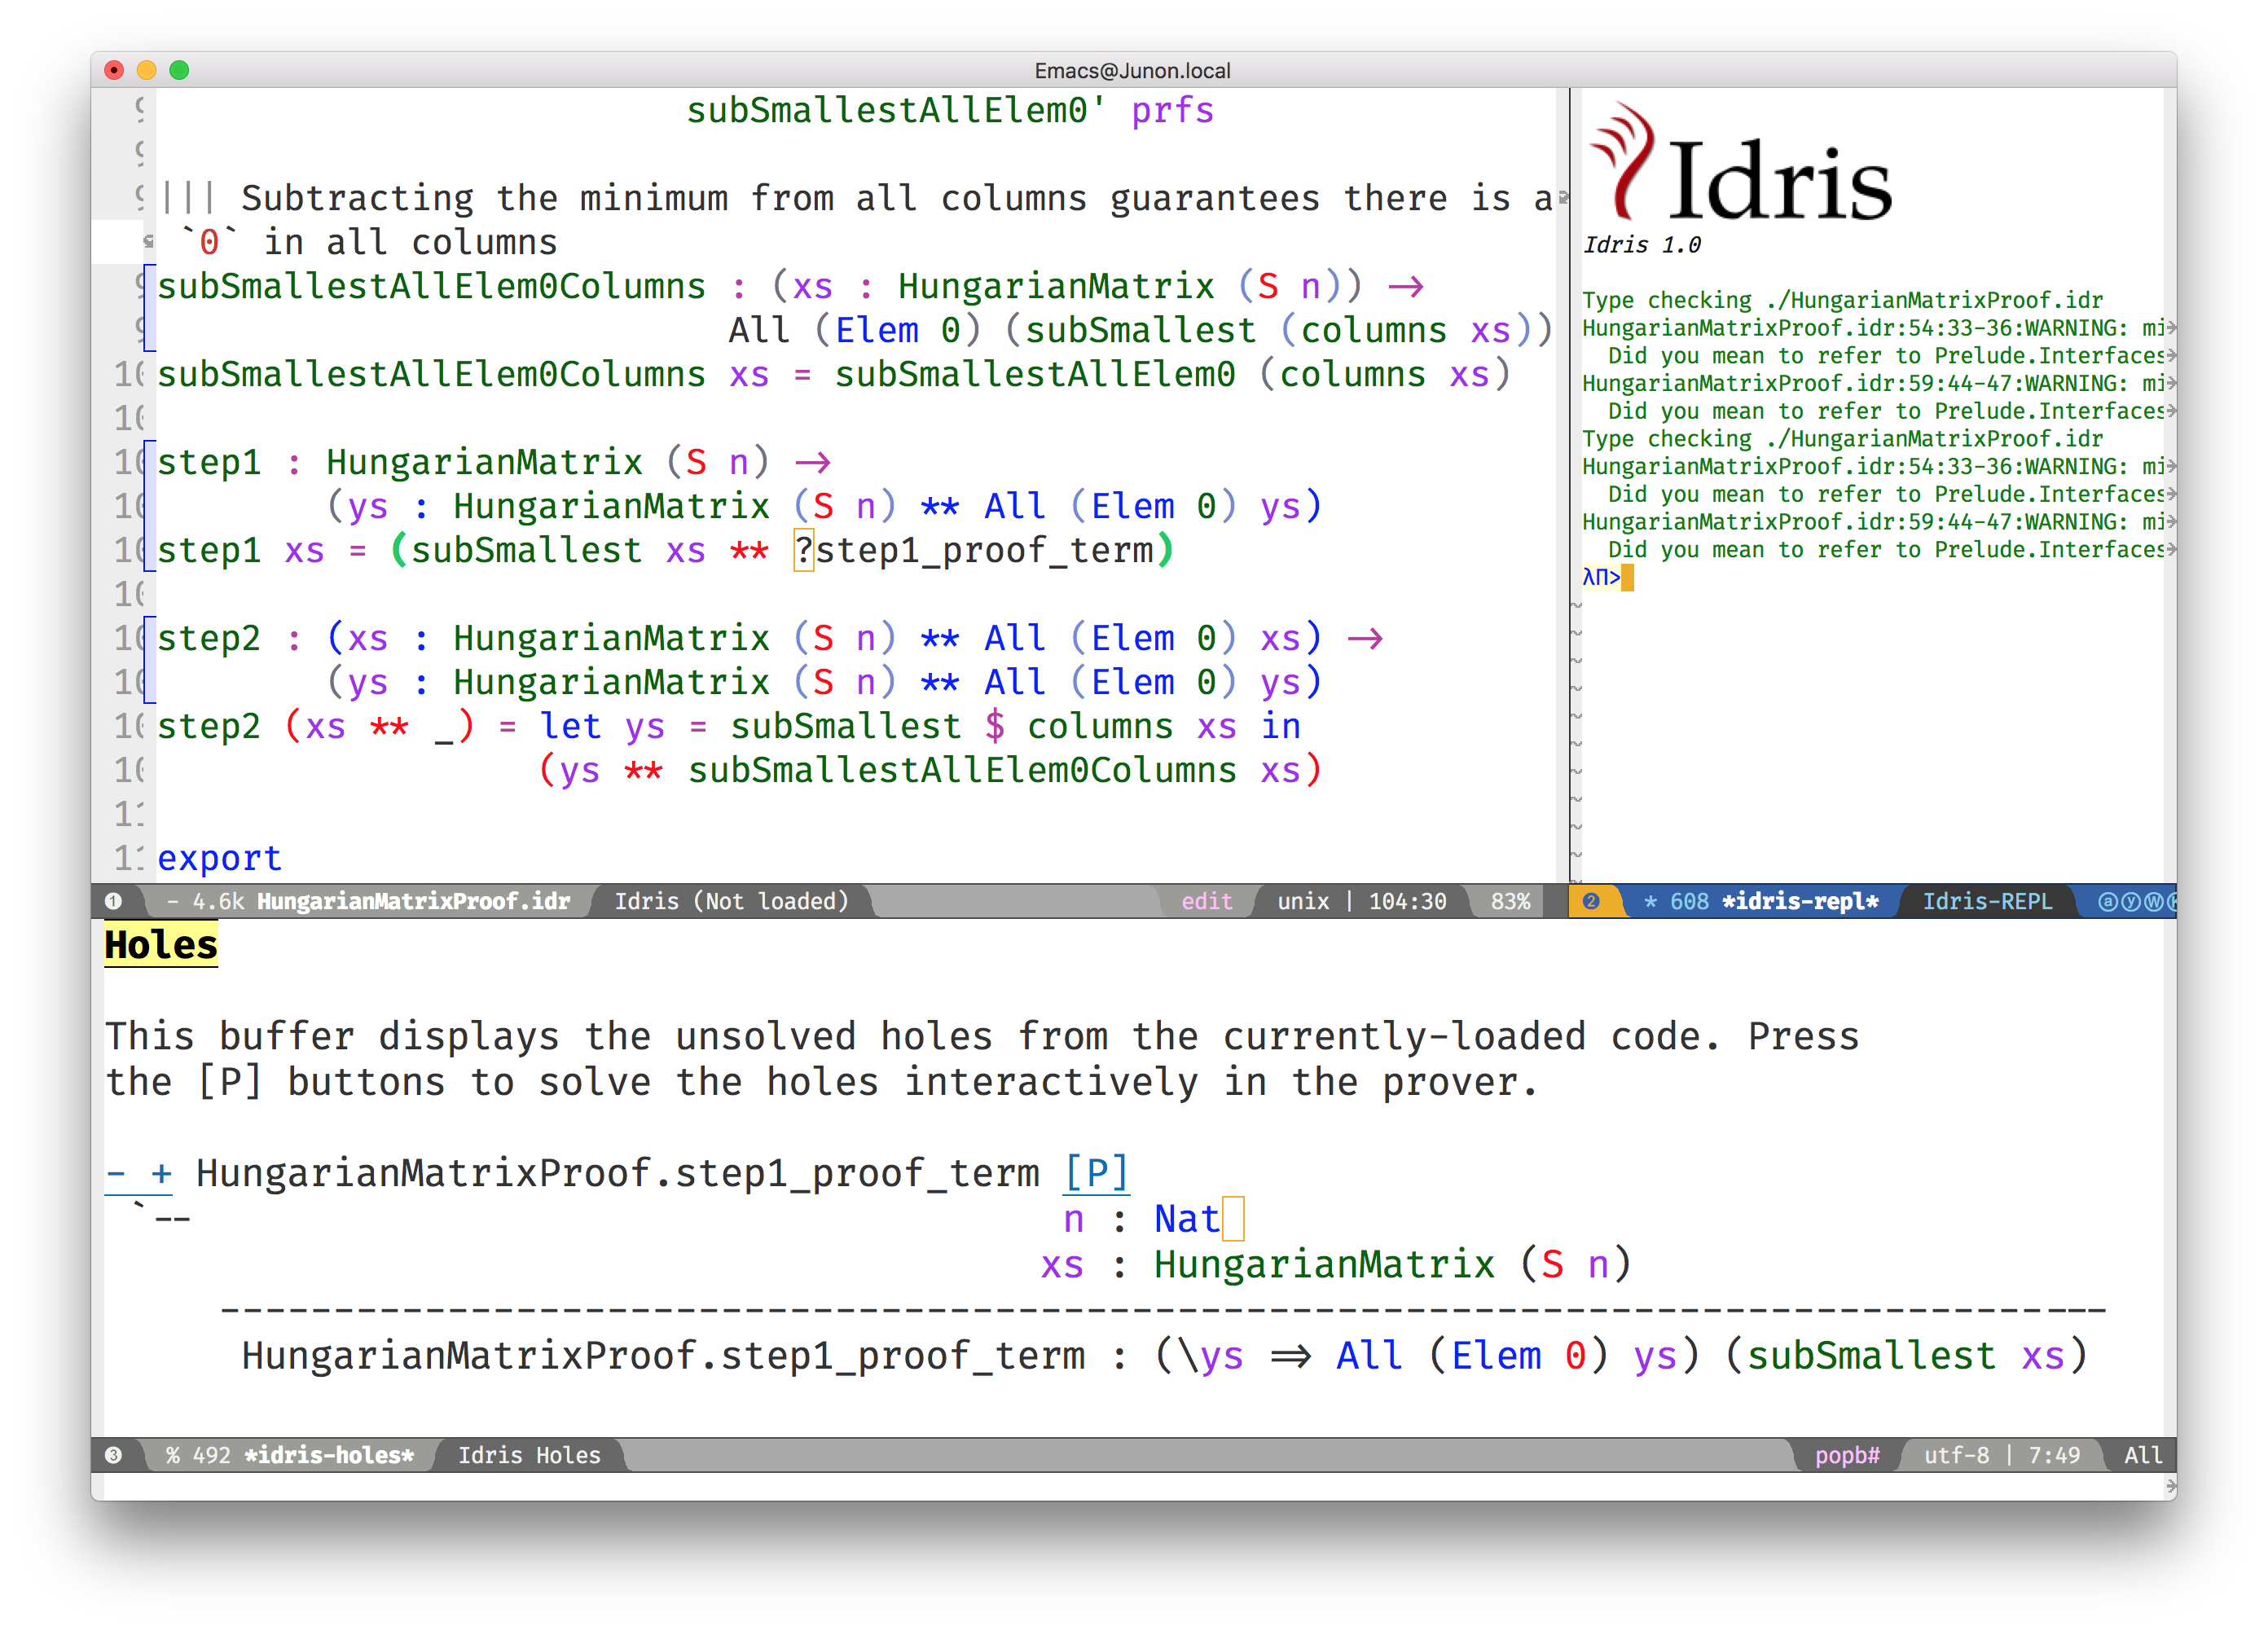
\includegraphics[width=0.85\linewidth]{./fig/interactive_idris.png}
\caption{An in-progress editing session using the interactive Idris mode}
\end{figure}

\section{Type-Driven Development}
\label{sec:orgee4028d}
The type-driven development approach is an iterative system for building up a
definition of a function or a set of functions using dependent types. The
approach is outlined, advocated and used throughout Edwin Brady's book
\cite{brady_book_2017} on Idris and this style of development. The approach
consists of three main steps:
\begin{enumerate}
\item Type
\item Define
\item Refine
\end{enumerate}

The first step, ``Type'', tells us to create an initial specification of what
the function should do by writing down the type we want it to have. The approach
is top-down from the type through to the function clauses in the definition. The
type serves as a specification that will help guide us towards a correct
implementation.

In the second step, ``Define'', we create an initial definition for the
function, possibly leaving in some typed holes. We do not yet know exactly how
to make our definition line up with the specification in the type so we use
holes to defer the actual implementation of the function. At this point we
should make use of as much knowledge as we know to the point where we can't
continue to implement the function. We can gain more information by making use
of features such as case splitting. We may also refer back to step one and
modify the type to continue with the process.

The third step, ``Refine'', is where we complete the function definition,
possibly modifying the type. This is the point where we use the other
definitions and functions available in our environment to complete our
type-checked definition according to our specification. We may at this point
realise also that our initial specification was incorrect or missing some piece
of information so that can lead us back to our first step in the cycle and we
can continue from there with a more rigorous type specification to drive our
implementation from.

\begin{figure}[H]
\centering
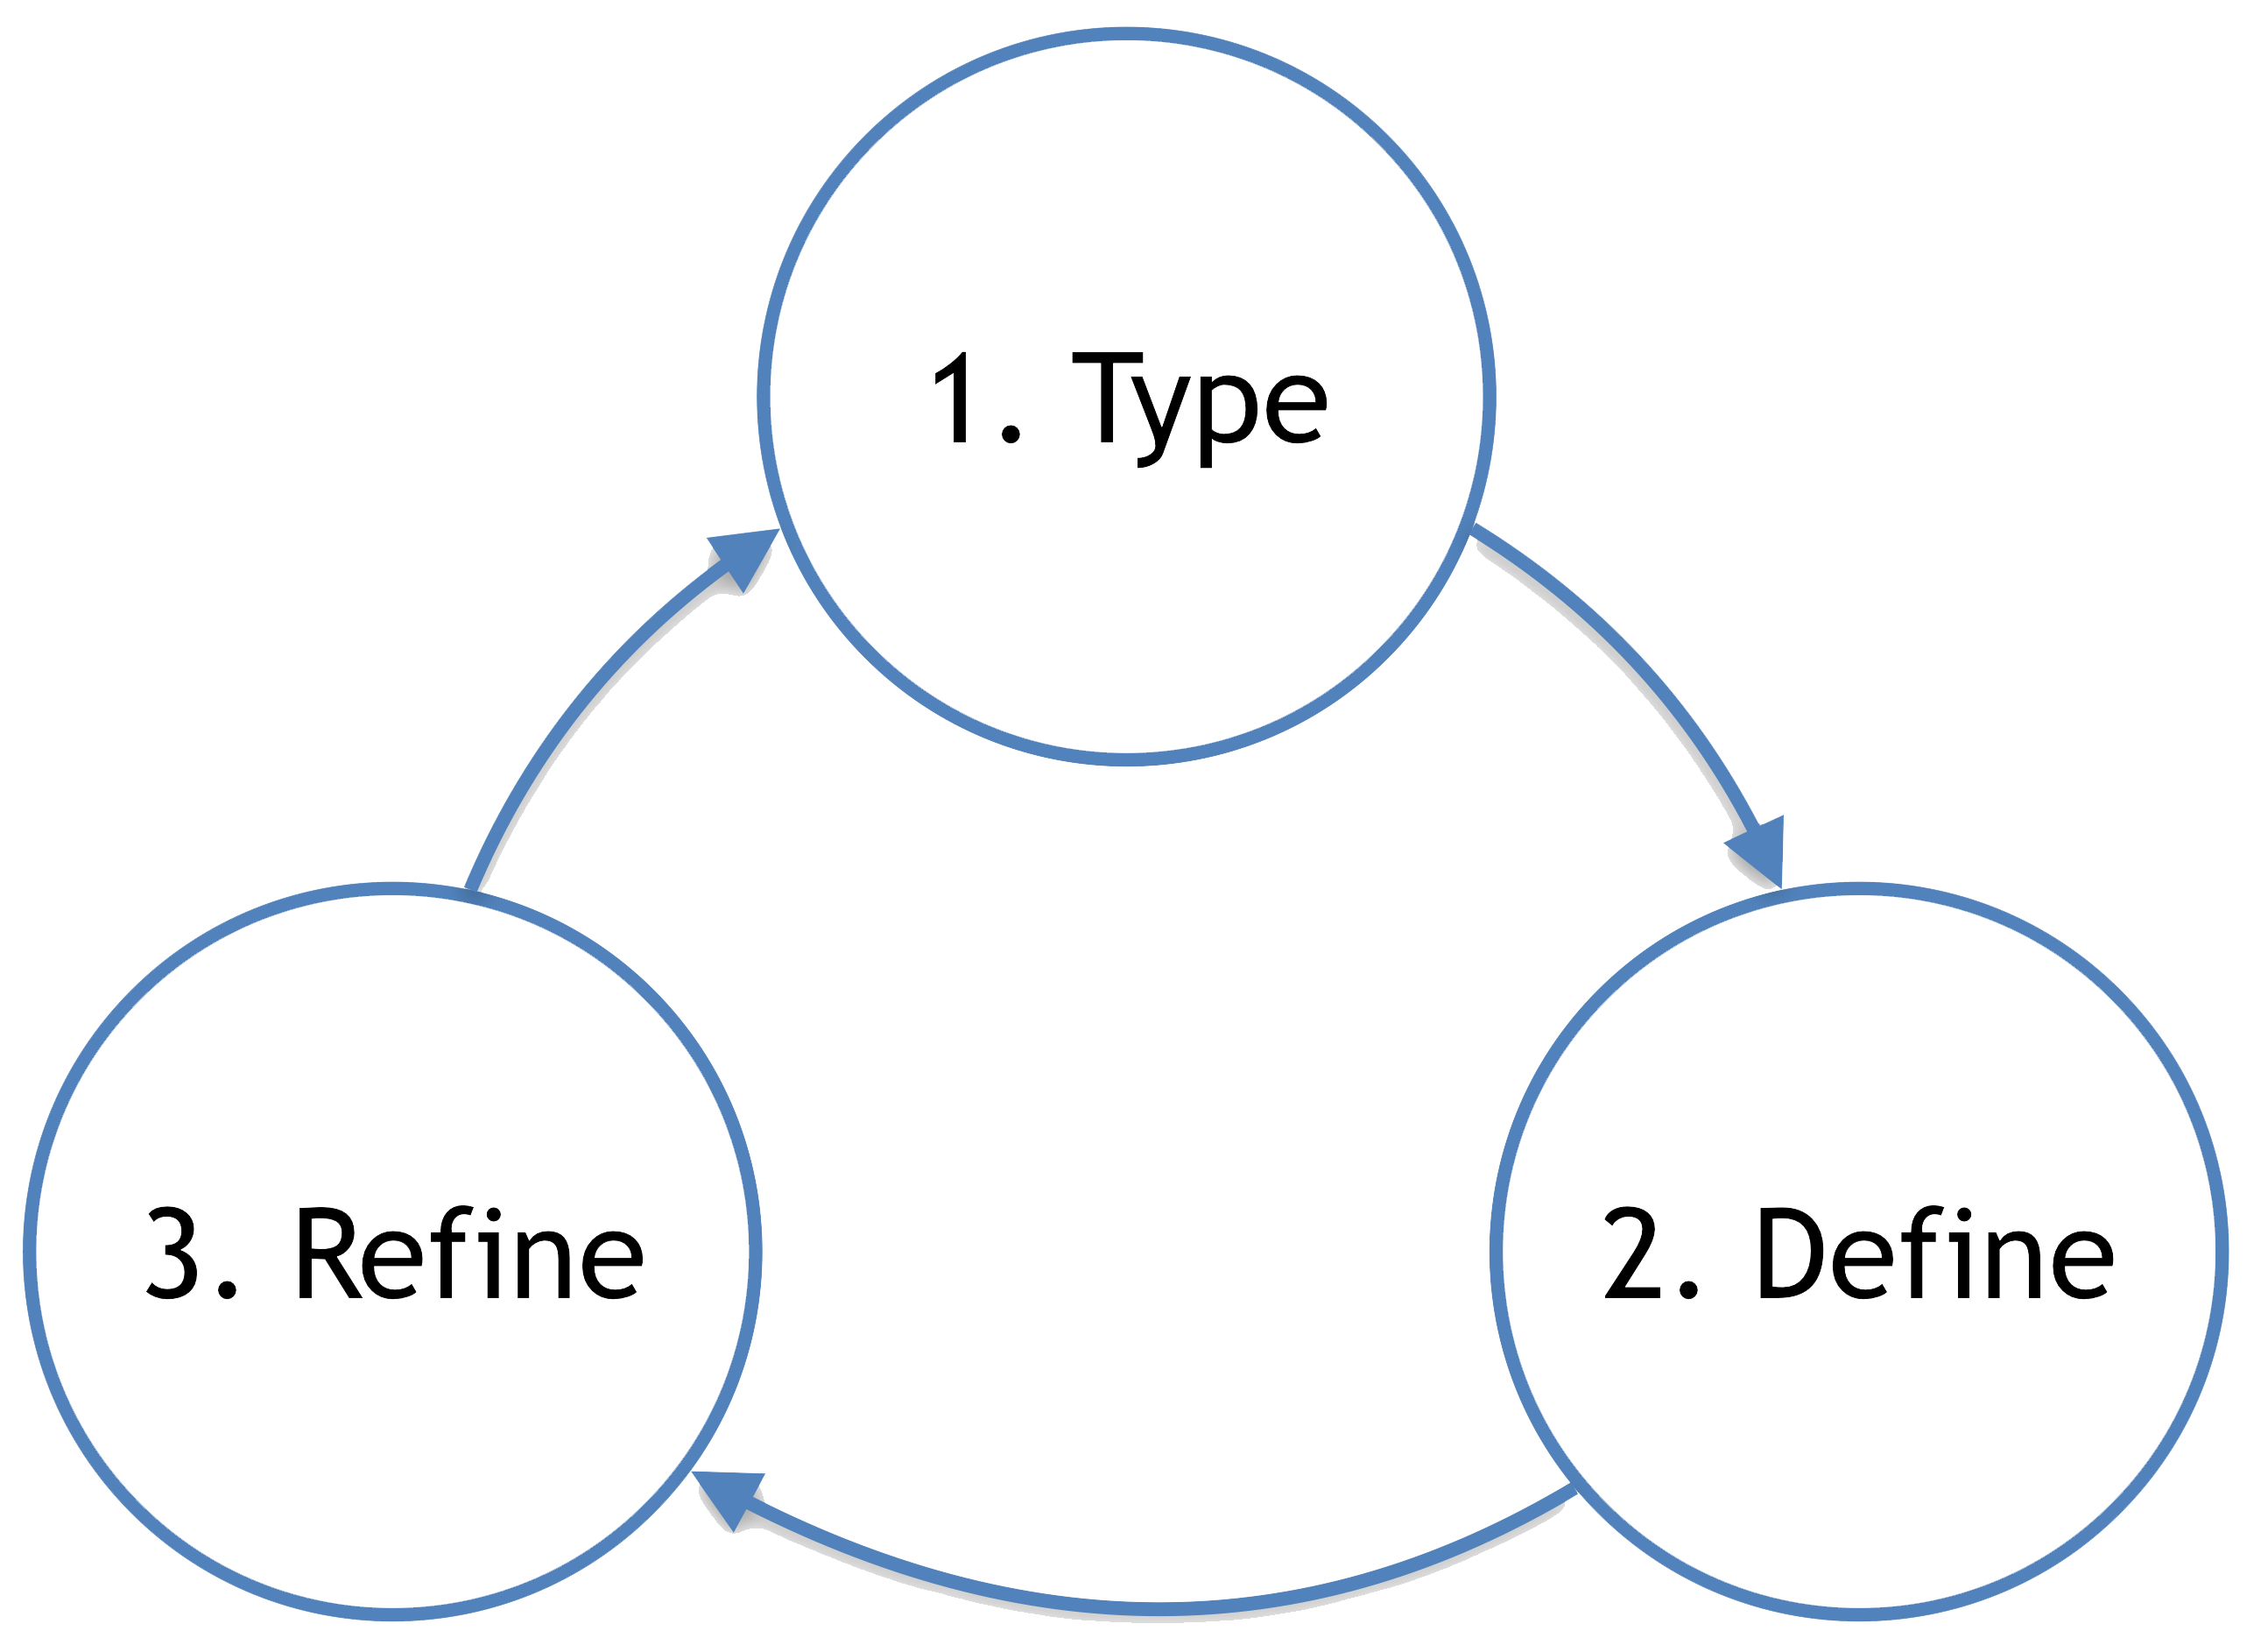
\includegraphics[width=0.8\linewidth]{./fig/tdd_cycle.png}
\caption{An illustration of the main workflow of the type-driven development approach}
\end{figure}

This style of development is greatly helped by the use of one of Idris'
interactive editing modes described earlier. In some cases the only manual
typing we might have to do is just writing our initial type specification. The
definition step in particular is aided. Using interactive editing modes we can
introduce an initial definition, case split on arguments and even try an initial
proof search on the typed holes we introduce. It may work out that the compiler
has everything it needs to create a correct type-checked definition without any
manual input from the user beyond the type of the function.

If we do need to provide more information, again, interactive editing helps get
us there. We can continue to inspect our environment to see the types of the
holes we need to define and also the environment of information available to us.
Reloading our modules and inspecting our current goals is one of the main
activities when programming in this type-driven fashion. As we continue to
refine our definition this type information also becomes refined and we can
continue to iterate over refining and modifying our types to reach a complete
definition.
\chapter{Case Studies}
\label{sec:org63969c1}
\chapter{Assessments and Conclusions}
\label{sec:org8f5cf4e}
\chapter{Future Work}
\label{sec:org8b77ee7}

\emergencystretch=1em
\printbibliography[heading=bibintoc, title=References]
\appendix
\end{document}